%Este trabalho está licenciado sob a Licença Atribuição-CompartilhaIgual 4.0 Internacional Creative Commons. Para visualizar uma cópia desta licença, visite http://creativecommons.org/licenses/by-sa/4.0/deed.pt_BR ou mande uma carta para Creative Commons, PO Box 1866, Mountain View, CA 94042, USA.

\chapter{Cônicas}\label{cap_conicas}
\thispagestyle{fancy}

\section{Elipse}\label{cap_conicas_sec_elipse}

Sejam $F_1,F_2$ pontos sobre um plano $\pi$, $c$ a distância entre $c_1$ e $c_2$ e $a > c$. Chama-se \emph{elipse} de \emph{focos} $F_1$ e $F_2$ ao conjunto de pontos $P$ tais que
\begin{equation}
  |PF_1| + |PF_2| = 2a.
\end{equation}
Veja a Figura \ref{fig:elipse}.

\begin{figure}[H]
  \centering
  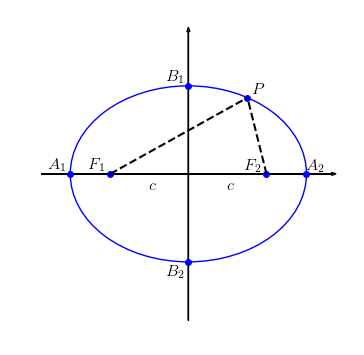
\includegraphics[width=0.7\textwidth]{./cap_conicas/dados/fig_elipse/fig_elipse}
  \caption{Ilustração de uma elipse de focos $F_1$ e $F_2$.}
  \label{fig:elipse}
\end{figure}

Dada uma tal elipse, identificamos $2c=|F_1F_2|$ como a \emph{distância focal}. Os pontos $A_1$ e $A_2$ de interseção da elipse com a reta que passa pelos focos são chamados de \emph{vértices} da elipse. O segmento $A_1A_2$ é chamado de \emph{eixo maior} da elipse. Observamos que
\begin{equation}
  |A_1A_2| = 2a.
\end{equation}
O ponto médio do segmento $F_1F_2$ é chamado de \emph{centro} da elipse. Sejam $B_1$ e $B_2$ os pontos de interseção da elipse com a reta que passa pelo centro da elipse e é perpendicular ao segmento $A_1A_2$. Assim sendo, o segmento $B_1B_2$ é chamado de \emph{eixo menor} da elipse. Vamos denotar
\begin{equation}
  2b = |B_1B_2|.
\end{equation}

Chamamos de \emph{excentricidade} da elipse o número
\begin{equation}
  e = \frac{c}{a}.
\end{equation}
Notemos que $0 \leq e < 1$. Para $e=0$, temos $c=0$ e, portanto $F_1=F_2$. Neste caso, a elipse é a circunferência de centro em $F_1$ (ou $F_2$) e diâmetro $2a$. No que $e$ tende a $1$, a elipse tende ao segmento $A_1A_2$.

Por fim, notemos que o triângulo $B_1OF_2$ é retângulo, $|OF_2|=c$, $|F_2B_1|=a$ e $|OB_1|=b$. Do teorema de Pitágoras segue
\begin{equation}\label{eq:elipse_obs}
  b^2 + c^2 = a^2.
\end{equation}

\subsection{Equação reduzida da elipse}

Consideremos o sistema de coordenadas cartesianas. Sejam $F_1=(-c,0)$ e $F_2=(c,0)$, $c\geq 0$, os focos de uma dada elipse (veja a Figura \ref{fig:elipse}).  Se $P=(x,y)$ é um ponto da elipse, então
\begin{equation}
  |PF_1| + |PF_2| = 2a.
\end{equation}
Como
\begin{align}
  |PF_1| &= \sqrt{(x+c)^2 + y^2}, \\
  |PF_2| &= \sqrt{(x-c)^2 + y^2},
\end{align}
temos
\begin{equation}
  \sqrt{(x+c)^2 + y^2} + \sqrt{(x-c)^2 + y^2} = 2a,
\end{equation}
ou, equivalentemente,
\begin{equation}
  \sqrt{(x+c)^2 + y^2} = 2a - \sqrt{(x-c)^2 + y^2}.
\end{equation}
Elevando ao quadrado, obtemos
\begin{equation}
  (x+c)^2 + y^2 = 4a^2 - 4a\sqrt{(x-c)^2+y^2} + (x-c)^2+y^2.
\end{equation}
Por cancelamento e rearranjo dos termos, obtemos
\begin{equation}
  a\sqrt{(x-c)^2+y^2}=a^2-cx.
\end{equation}
Elevando novamente ao quadrado, temos
\begin{equation}
  a^2(x-c)^2+a^2y^2=a^4-2a^2cx+c^2x^2,
\end{equation}
donde
\begin{equation}
  a^2x^2 -2a^2cx + a^2c^2 + a^2y^2= a^4 -2a^2cx + c^2x^2.
\end{equation}
Por cancelamento e rearranjo dos termos, obtemos
\begin{equation}
  x^2(a^2 - c^2) + a^2y^2 = a^2(a^2 - c^2).
\end{equation}
Como $a>c$, dividimos por $a^2-c^2$  e depois por $a^2$ para obtemos
\begin{equation}
  \frac{x^2}{a^2} + \frac{y^2}{a^2-c^2} = 1.
\end{equation}
Por fim, da equação \eqref{eq:elipse_obs}, temos $a^2-c^2 = b^2$, o que nos leva  a \emph{equação reduzida da elipse}
\begin{equation}
  \frac{x^2}{a^2} - \frac{y^2}{b^2} = 1.
\end{equation}

\subsection*{Exercícios resolvidos}

\emconstrucao

\subsection*{Exercícios}

\emconstrucao

\section{Hipérbole}\label{cap_conicas_sec_hiperbole}

Sejam $F_1$ e $F_2$ pontos sobre um plano $\pi$ e. Sejam, também, $c$ tal que $|F_1F_2|=2c$ e $a<c$. O lugar geométrico dos pontos $P$ tais que
\begin{equation}
  ||PF_1|-|PF_2||=2a,
\end{equation}
chama-se \pmb{hipérbole}. Veja Figura \ref{fig:hiperbole}.

\begin{figure}[H]
  \centering
  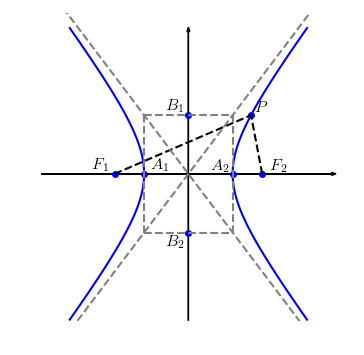
\includegraphics[width=0.7\textwidth]{./cap_conicas/dados/fig_hiperbole/fig_hiperbole}
  \caption{Ilustração de uma hipérbole de focos $F_1$ e $F_2$.}
  \label{fig:hiperbole}
\end{figure}

Os pontos $F_1$ e $F_2$ são chamados de \emph{focos} da hipérbole e $2c = |F_1F_2|$ é chamada de \emph{distância focal}. O ponto médio entre os pontos $F_1$ e $F_2$ é chamado de centro da hipérbole. São chamados \emph{vértices} da hipérbole os pontos $A_1$ e $A_2$, sendo que o segmento $A_1A_2$ é chamado de \emph{eixo real} (ou transverso) da hipérbole. O comprimento deste eixo é $|A_1A_2|=2a$.

Sejam $B_1$ e $B_2$ pontos $c$ distantes de $A_1$ e $A_2$ e pertencentes a reta que passa pelo centro da hipérbole e é perpendicular ao seu eixo real. O segmento $B_1B_2$ é chamado de \emph{eixo imaginário} (transverso ou conjugado). Denotando $2b=|B_1B_2|$, temos do triângulo retângulo $B_1OA_1$ que
\begin{equation}
  c^2 = a^2 + b^2.
\end{equation}

\subsection{Equação reduzida da hipérbole}

Assumimos um sistema de coordenadas cujo centro coincida com o centro de uma dada hipérbole e o eixo das abscissas seja coincidente com o eixo real da hipérbole. Desta forma, temos $F_1 = (-c,0)$ e $F_2 = (c,0)$. Então, $P=(x,y)$ é um ponto da hipérbole quando
\begin{equation}
  ||PF_1|-|PF_2|| = 2a.
\end{equation}
Daí, segue que
\begin{align}
  |PF_1|-|PF_2| &= \pm 2a \Rightarrow \sqrt{(x+c)^2+y^2}-\sqrt{(x-c)^2+y^2}=\pm 2a\\
                &\Rightarrow \sqrt{(x+c)^2+y^2} = \pm 2a + \sqrt{(x-c)^2+y^2}.
\end{align}
Elevando ao quadrado ambos os lados desta última equação, obtemos
\begin{equation}
  (x+c)^2+y^2 = 4a^2 \pm 4a\sqrt{(x-c)^2+y^2} + (x-c)^2+y^2
\end{equation}
ou, equivalentemente,
\begin{equation}
  x^2+2cx+c^2+y^2=4a^2\pm4a\sqrt{(x-c)^2+y^2}+x^2-2cx+c^2+y^2.
\end{equation}
Simplificando e rearranjando os termos, temos
\begin{equation}
  cx - a^2 = \pm a\sqrt{(x-c)^2+y^2}).
\end{equation}
Elevando novamente ao quadrado, obtemos
\begin{equation}
  c^2x^2 - 2a^2cx + a^4 = a^2x^2 - 2a^2cx + a^2c^2 + a^2y^2.
\end{equation}
Simplificando e rearranjando os termos, obtemos
\begin{equation}
  (c^2-a^2)x^2 - a^2y^2 = a^2(c^2-a^2).
\end{equation}
Lembrando que $c^2 = a^2 + b^2$, temos
\begin{equation}
  b^2x^2 - a^2y^2 = a^2b^2.
\end{equation}
Dividindo por $a^2b^2$, obtemos
\begin{equation}
  \frac{x^2}{a^2} - \frac{y^2}{b^2} = 1,
\end{equation}
a qual é chamada de \emph{equação reduzida da hipérbole}.

\emconstrucao

\section{Parábola}\label{cap_conicas_sec_parabola}

Em um plano, consideramos uma reta $d$ e um ponto $F$ não pertencente a $d$. Chamamos de \emph{parábola} o conjunto de pontos $P$ do plano que são equidistantes de $F$ e de $d$, i.e.
\begin{equation}
  \dist(P,F) = \dist(P,d).
\end{equation}
Veja a Figura \ref{fig:parabola}.

\begin{figure}[H]
  \centering
  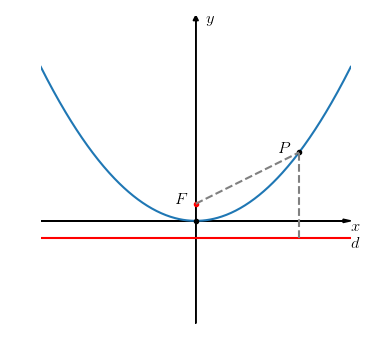
\includegraphics[width=0.7\textwidth]{./cap_conicas/dados/fig_parabola/fig_parabola}
  \caption{Ilustração de uma parábola.}
  \label{fig:parabola}
\end{figure}

O ponto $F$ é chamado de \emph{foco} da parábola. A reta $d$ é chamada de \emph{diretriz} da parábola. A reta perpendicular a $d$ e que passa pelo ponto $F$ é chamada de \emph{eixo} da parábola. O ponto $V$ de interseção entre a parábola e seu eixo é chamado de \emph{vértice} da parábola.

\subsection{Equação reduzida de uma parábola}

Tomamos o sistema cartesiano de coordenadas com origem no vértice da parábola e eixo das abscissas paralelo à diretriz. Seja $p$ tal que
\begin{equation}
  F = (0,p/2).
\end{equation}
Logo, a diretriz tem equação $y = -p/2$. Da definição de parábola, $P=(x,y)$ pertence a parábola quando
\begin{equation}
  \dist(P,F) = \dist(P,d).
\end{equation}
Segue que
\begin{equation}
  \sqrt{x^2+\left(y-\frac{p}{2}\right)^2} = y+\frac{p}{2}.
\end{equation}
Elevando ao quadrado e expandindo, obtemos
\begin{equation}
  x^2 + y^2-py+\frac{p^2}{4} = y^2 + py + \frac{p^2}{4}.
\end{equation}
Cancelando e rearranjando termos, obtemos
\begin{equation}
  x^2 = 2py,
\end{equation}
a chamada \emph{equação reduzida da parábola}.

\begin{obs}
  Uma parábola com vértice na origem do sistema cartesiano e foco $F=(p/2, 0)$, tem equação reduzida
  \begin{equation}
    y^2 = 2px.
  \end{equation}
\end{obs}

\subsection*{Exercícios resolvidos}

\emconstrucao

\subsection*{Exercícios}

\emconstrucao